\chapter{MEMS逆向光调制器(MRR)}
常用的逆光调制器如图~\ref{DIFF-MRR-CMP.pdf}所示。
\addimg{1}{DIFF-MRR-CMP.pdf}{常用的逆向光调制器MRR}

从图~\ref{DIFF-MRR-CMP.pdf}中可以看出铁电液晶调制器通信速率上限不高,而且体积大,不利于在小型平台上的应用;电光调制器虽然调制速率可以做得很高,但是所需的控制电压很高,不利于进行功耗控制,无法在固定容量的电池下,长时间的工作;相对前面两款,MEMS因为驱动电压低,体积紧凑,调制速率满足基本的需求,功耗低因而目前应用很广泛,很有潜力;最有为了克服MEMS调制器通信距离受限的缺点,有研究者考虑在MEMS调制器后端接光纤放大器,对信号进行二次放大后反射回探测器,使得传输距离大大提高。



\section{MEMS逆向光调制器的工作原理}
\addimg{1}{BOSTON-MRR-PRICNPLE.jpg}{MEMS逆向光调制器工作示意图}
典型的MEMS逆光调制器原理如图~\ref{MEMS-MRR.pdf},这种模式主要工作于OOK模式,即通过是否施加电压以改变镜面的形状,如图~\ref{fig:mems-principle.pdf}。当施加电压为零时,MEMS器件表面平整,询问光束照射后,以镜面反射的形式返回给主动端,表示“1”状态;当施加电压为非零值时,MEMS器件表面变得粗糙,很多沟槽出现,询问光束照射后,发生漫反射,很少光线能返回主动端,表示“0”状态,如图~\ref{fig:MRR-TWO-STATE.pdf}。

\addimg{1}{MEMS-MRR.pdf}{典型的MEMS逆光调制器原理}
%\addimg{1}{mems-principle.pdf}{MEMS逆向调制器的工作原理}
%
%\addimg{1}{MRR-TWO-STATE.pdf}{MEMS逆向调制器工作的两种状态}
\begin{figure}[!htbp]
	\centering
	\begin{subfigure}[c]{0.5\textwidth}
		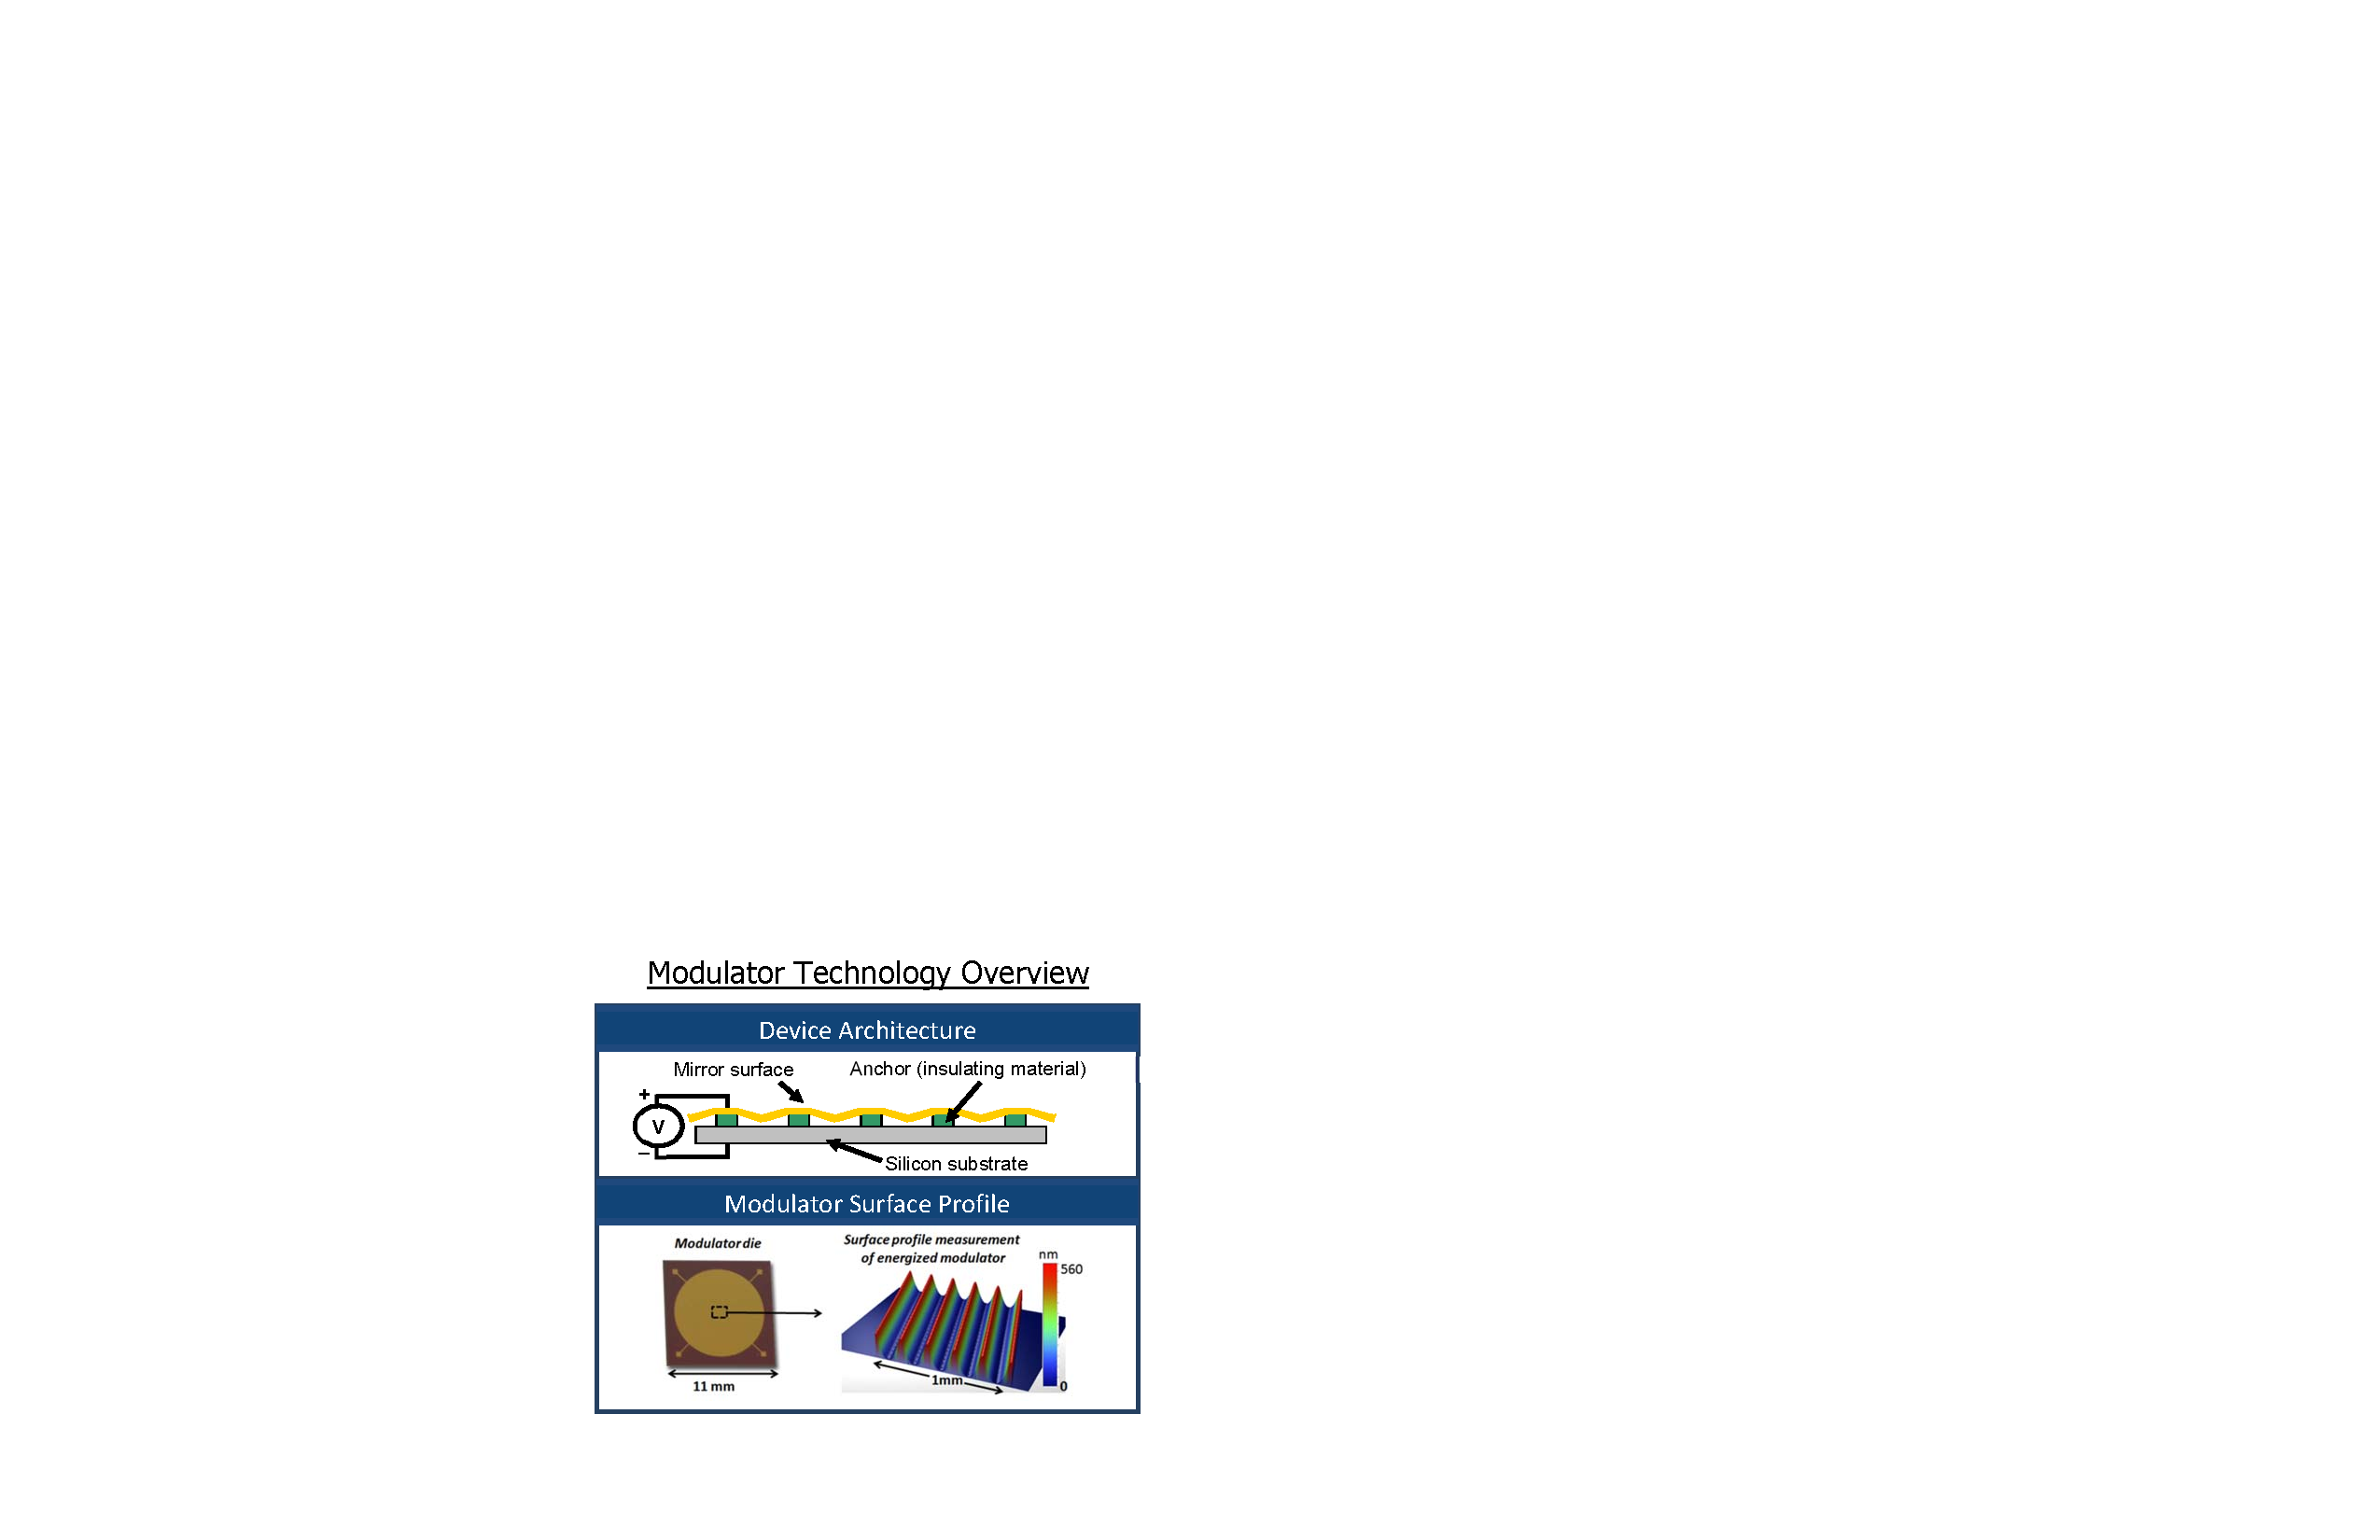
\includegraphics[width=\textwidth]{./Img/mems-principle.pdf}
		\caption{}
		\label{fig:mems-principle.pdf}
	\end{subfigure}%
	~%add desired spacing
	\begin{subfigure}[c]{0.5\textwidth}
		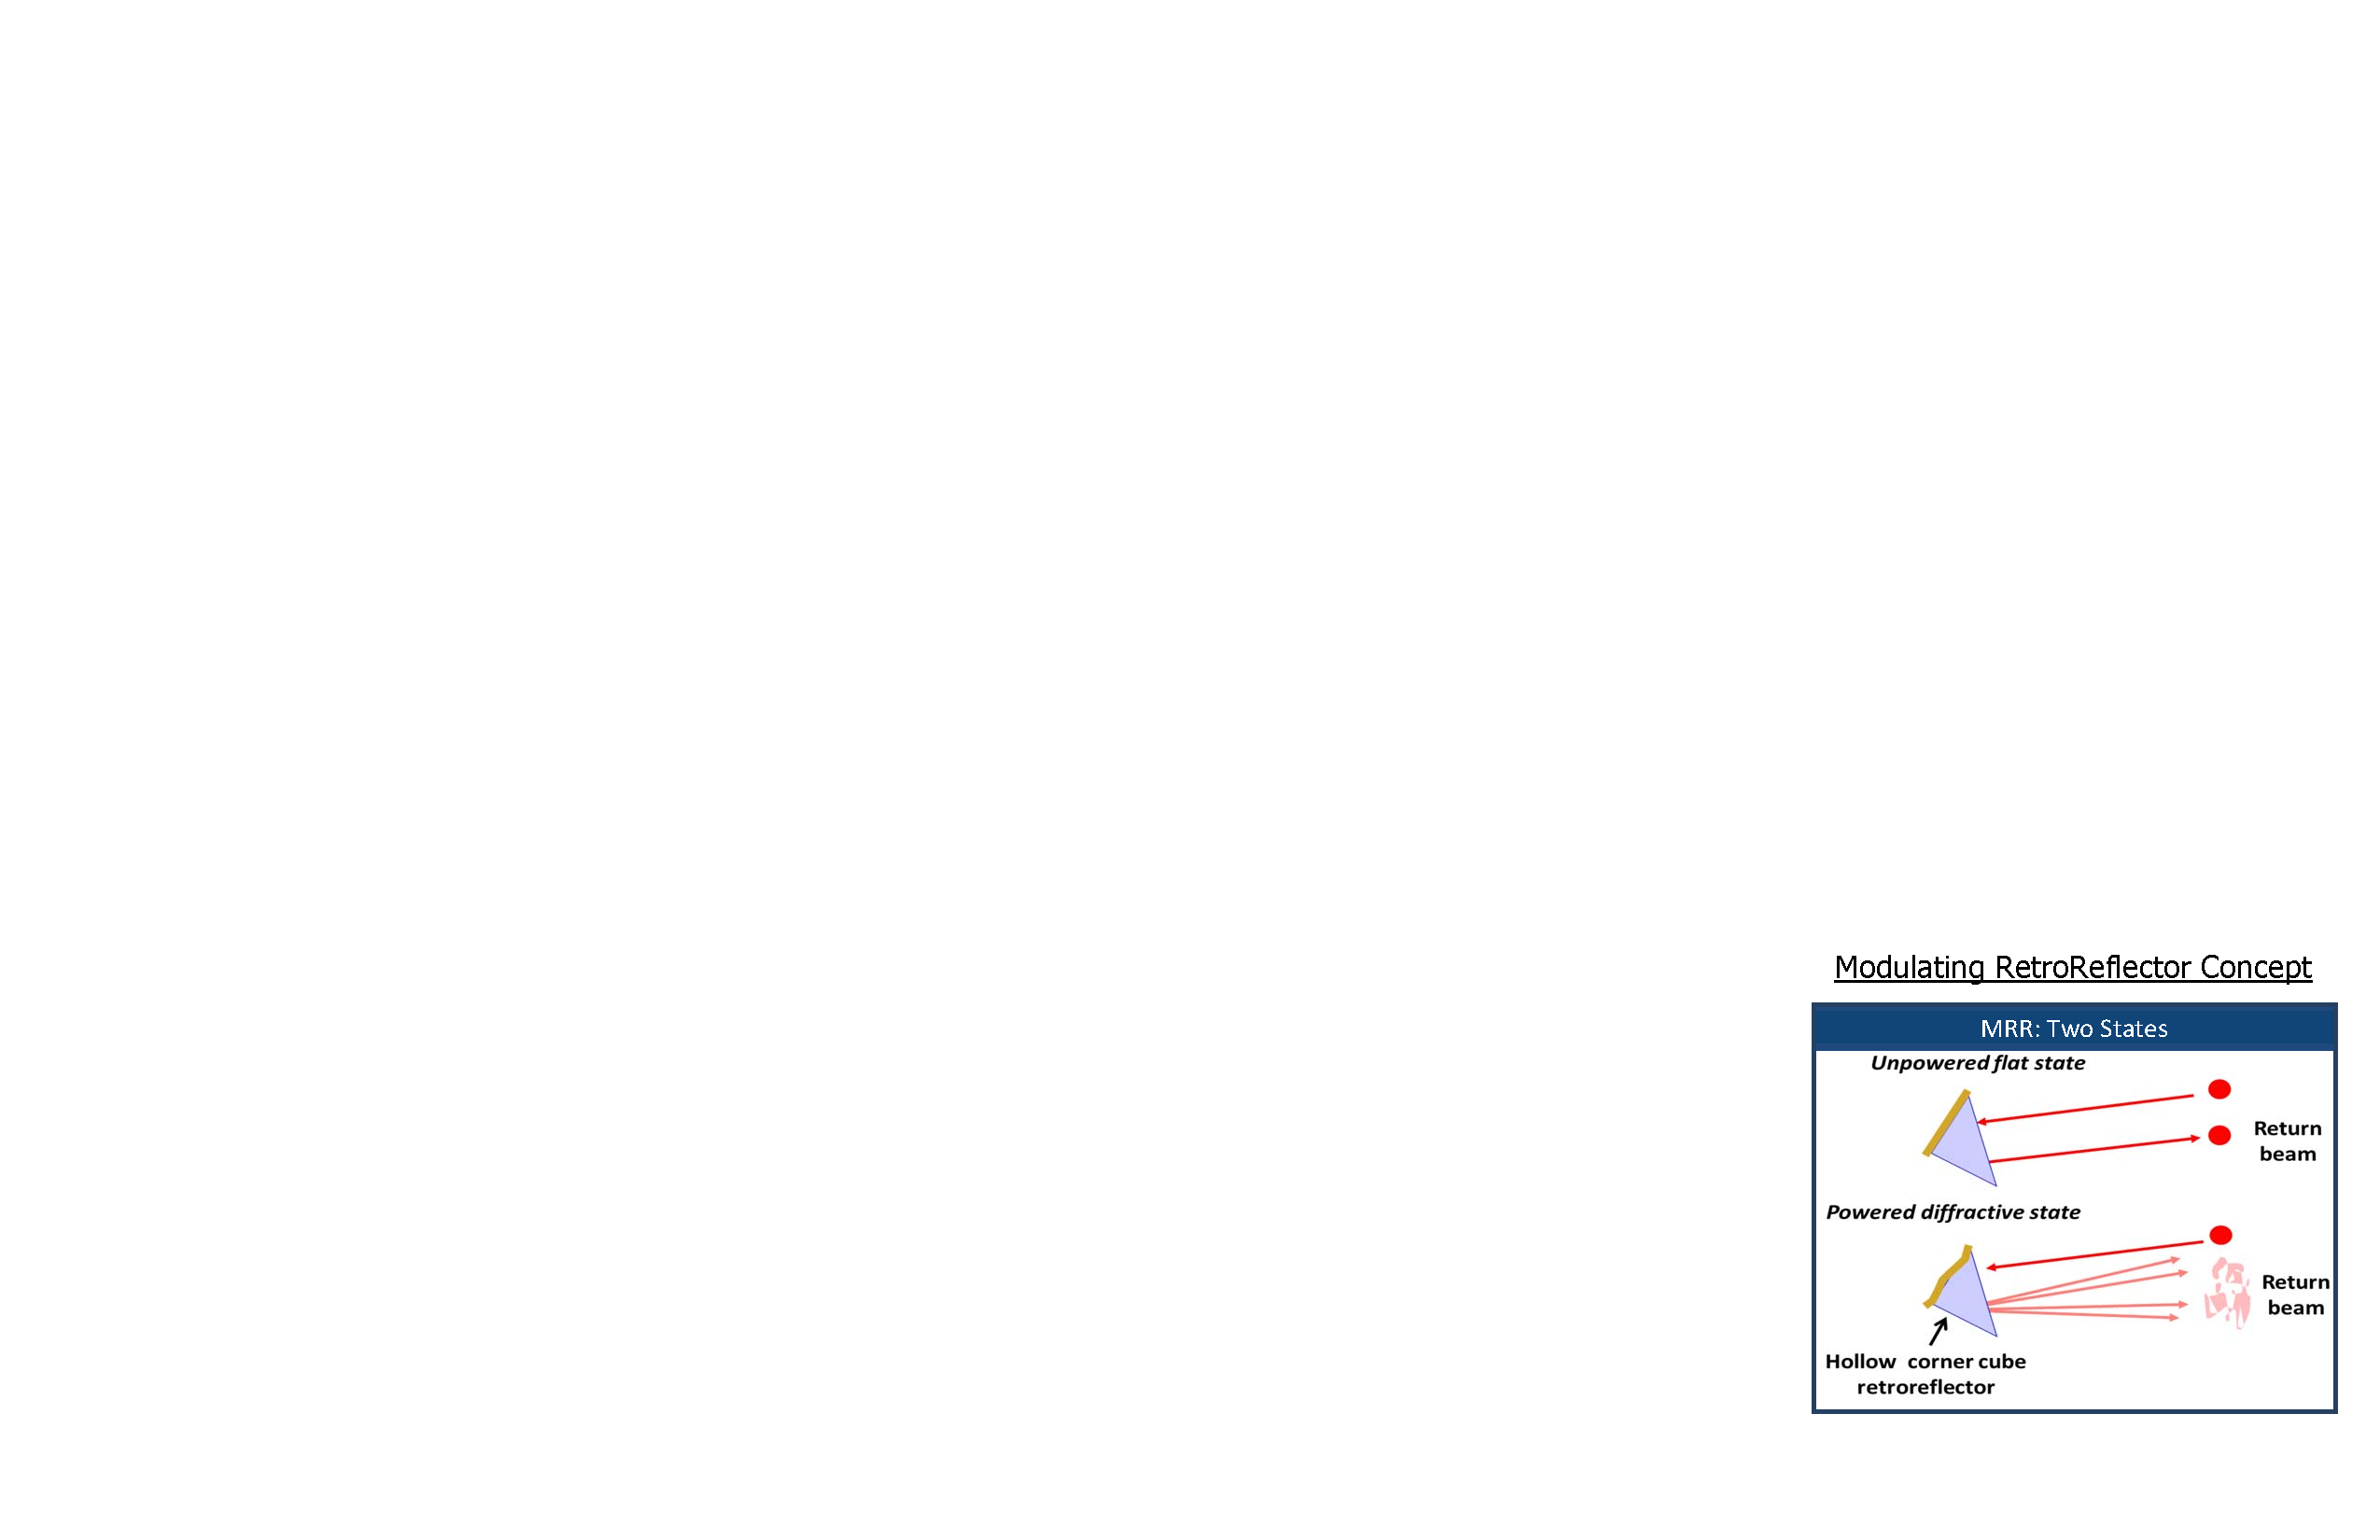
\includegraphics[width=\textwidth]{./Img/MRR-TWO-STATE.pdf}
		\caption{}
		\label{fig:MRR-TWO-STATE.pdf}
	\end{subfigure}
	\bicaption{MEMS逆光调制器。(a) MEMS逆向调制器的工作原理,(b) MEMS微镜的两种工作状态}{MEMS MRR.(a) MEMS -MRR-principle , (b) MRR-TWO-STATE }
	\label{fig:MEMS-MRR-manual}
\end{figure}

该MEMS逆向光调制工作频宽,可在从可见光到中红外的广泛波长范围内工作。它是一种具有反射式衍射光栅,通过驱动器施加电压控制(如图~\ref{fig:boston-MEMS-MRR-driver.jpg}),即可控制凹槽深度,其最大深度取决于基体电极槽的深度,如图~\ref{fig:mems-principle.pdf}。

\section{MEMS逆向光调制器}
\subsection{产品概述}
波士顿微机械公司(Boston Micromachines)开创了MEMS(微机电系统)变形镜技术,用于先进的光学控制。这些微型精密的光塑形器使世界顶尖的研究人员能够在天文学、显微学、激光控制和视网膜成像方面取得突破。在MEMS镜像技术的发展和向全高分辨率成像系统的扩展方面,波士顿微机械公司处于行业领先地位,致力于推动光子学应用领域的发现。

波士顿微机械公司对于逆向光通信推出了两款微镜,分别是镜面分立型MEMS(\ref{fig:Segmented-DM.png})和镜面连续型MEMS(图~\ref{fig:Continuous-DM.png})。

%\addimg{1}{Segmented-DM.png}{MEMS分立微镜示意图}
%\addimg{1}{Continuous-DM.png}{MEMS连续微镜示意图}
\begin{figure}[!htbp]
	\centering
	\begin{subfigure}[c]{0.5\textwidth}
	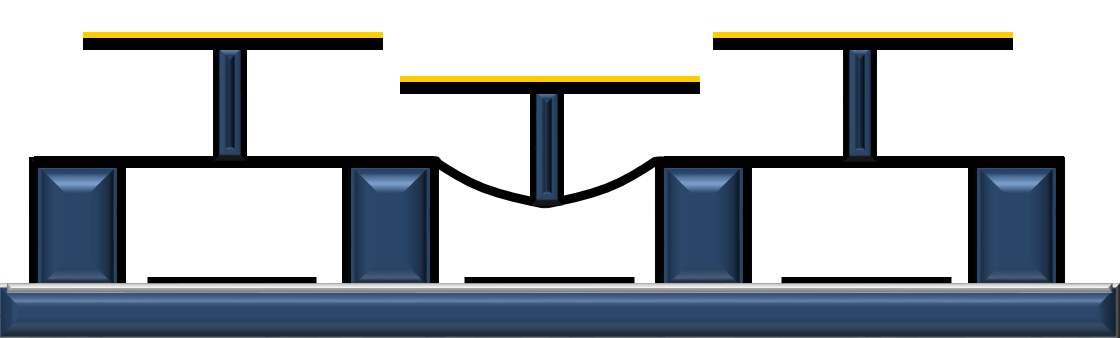
\includegraphics[width=\textwidth]{./Img/Segmented-DM.png}
	\caption{}
	\label{fig:Segmented-DM.png}
	\end{subfigure}%
	~%add desired spacing
	\begin{subfigure}[c]{0.5\textwidth}
	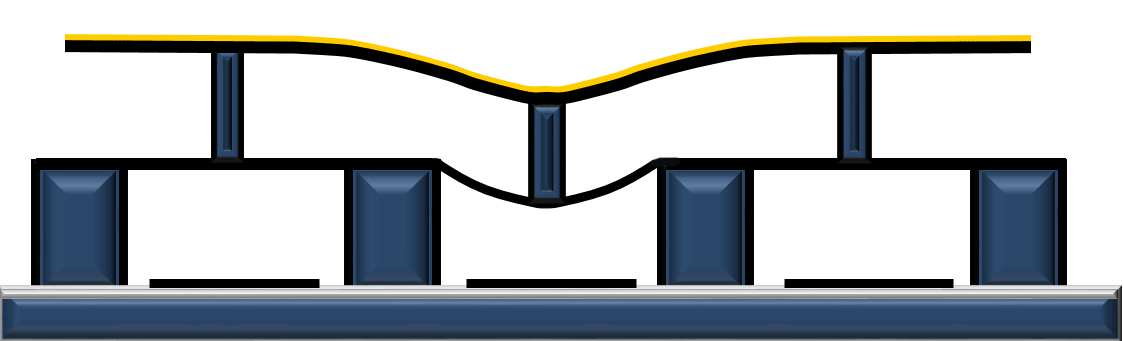
\includegraphics[width=\textwidth]{./Img/Continuous-DM.png}
		\caption{}
		\label{fig:Continuous-DM.png}
	\end{subfigure}
	\bicaption{MEMS逆光调制器。(a) MEMS分立微镜示意图,(b) MEMS连续微镜示意图}{MEMS MRR.(a) Segmented-DM , (b) Continuous-DM }
\label{fig:MEMS-MRR}
\end{figure}


%\addimg{1}{boston-MEMS-MRR-driver.jpg}{MEMS逆向调制器驱动器}
%\addimg{1}{boston-MEMS-MRR-INNER.jpg}{MEMS逆向调制器内部结构图}
%\addimg{1}{boston-MEMS-MRR-outer.jpg}{MEMS逆向调制器外型图}
\begin{figure}[!htbp]
	\centering
	\begin{subfigure}[c]{0.3\textwidth}
		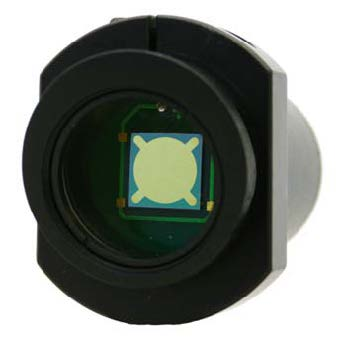
\includegraphics[width=\textwidth]{./Img/boston-MEMS-MRR-INNER.jpg}
		\caption{}
		\label{fig:boston-MEMS-MRR-INNER.jpg}
	\end{subfigure}%
	~%add desired spacing
	\begin{subfigure}[c]{0.3\textwidth}
		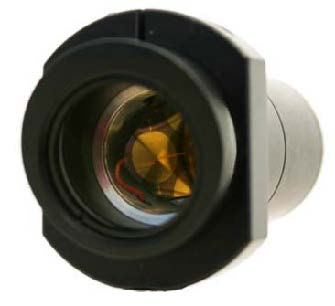
\includegraphics[width=\textwidth]{./Img/boston-MEMS-MRR-outer.jpg}
		\caption{}
		\label{fig:boston-MEMS-MRR-outer.jpg}
	\end{subfigure}
	\begin{subfigure}[c]{0.3\textwidth}
		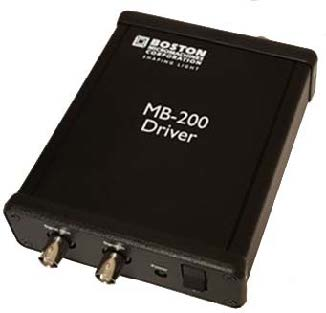
\includegraphics[width=\textwidth]{./Img/boston-MEMS-MRR-driver.jpg}
		\caption{}
		\label{fig:boston-MEMS-MRR-driver.jpg}
	\end{subfigure}
	\begin{subfigure}[c]{1\textwidth}
	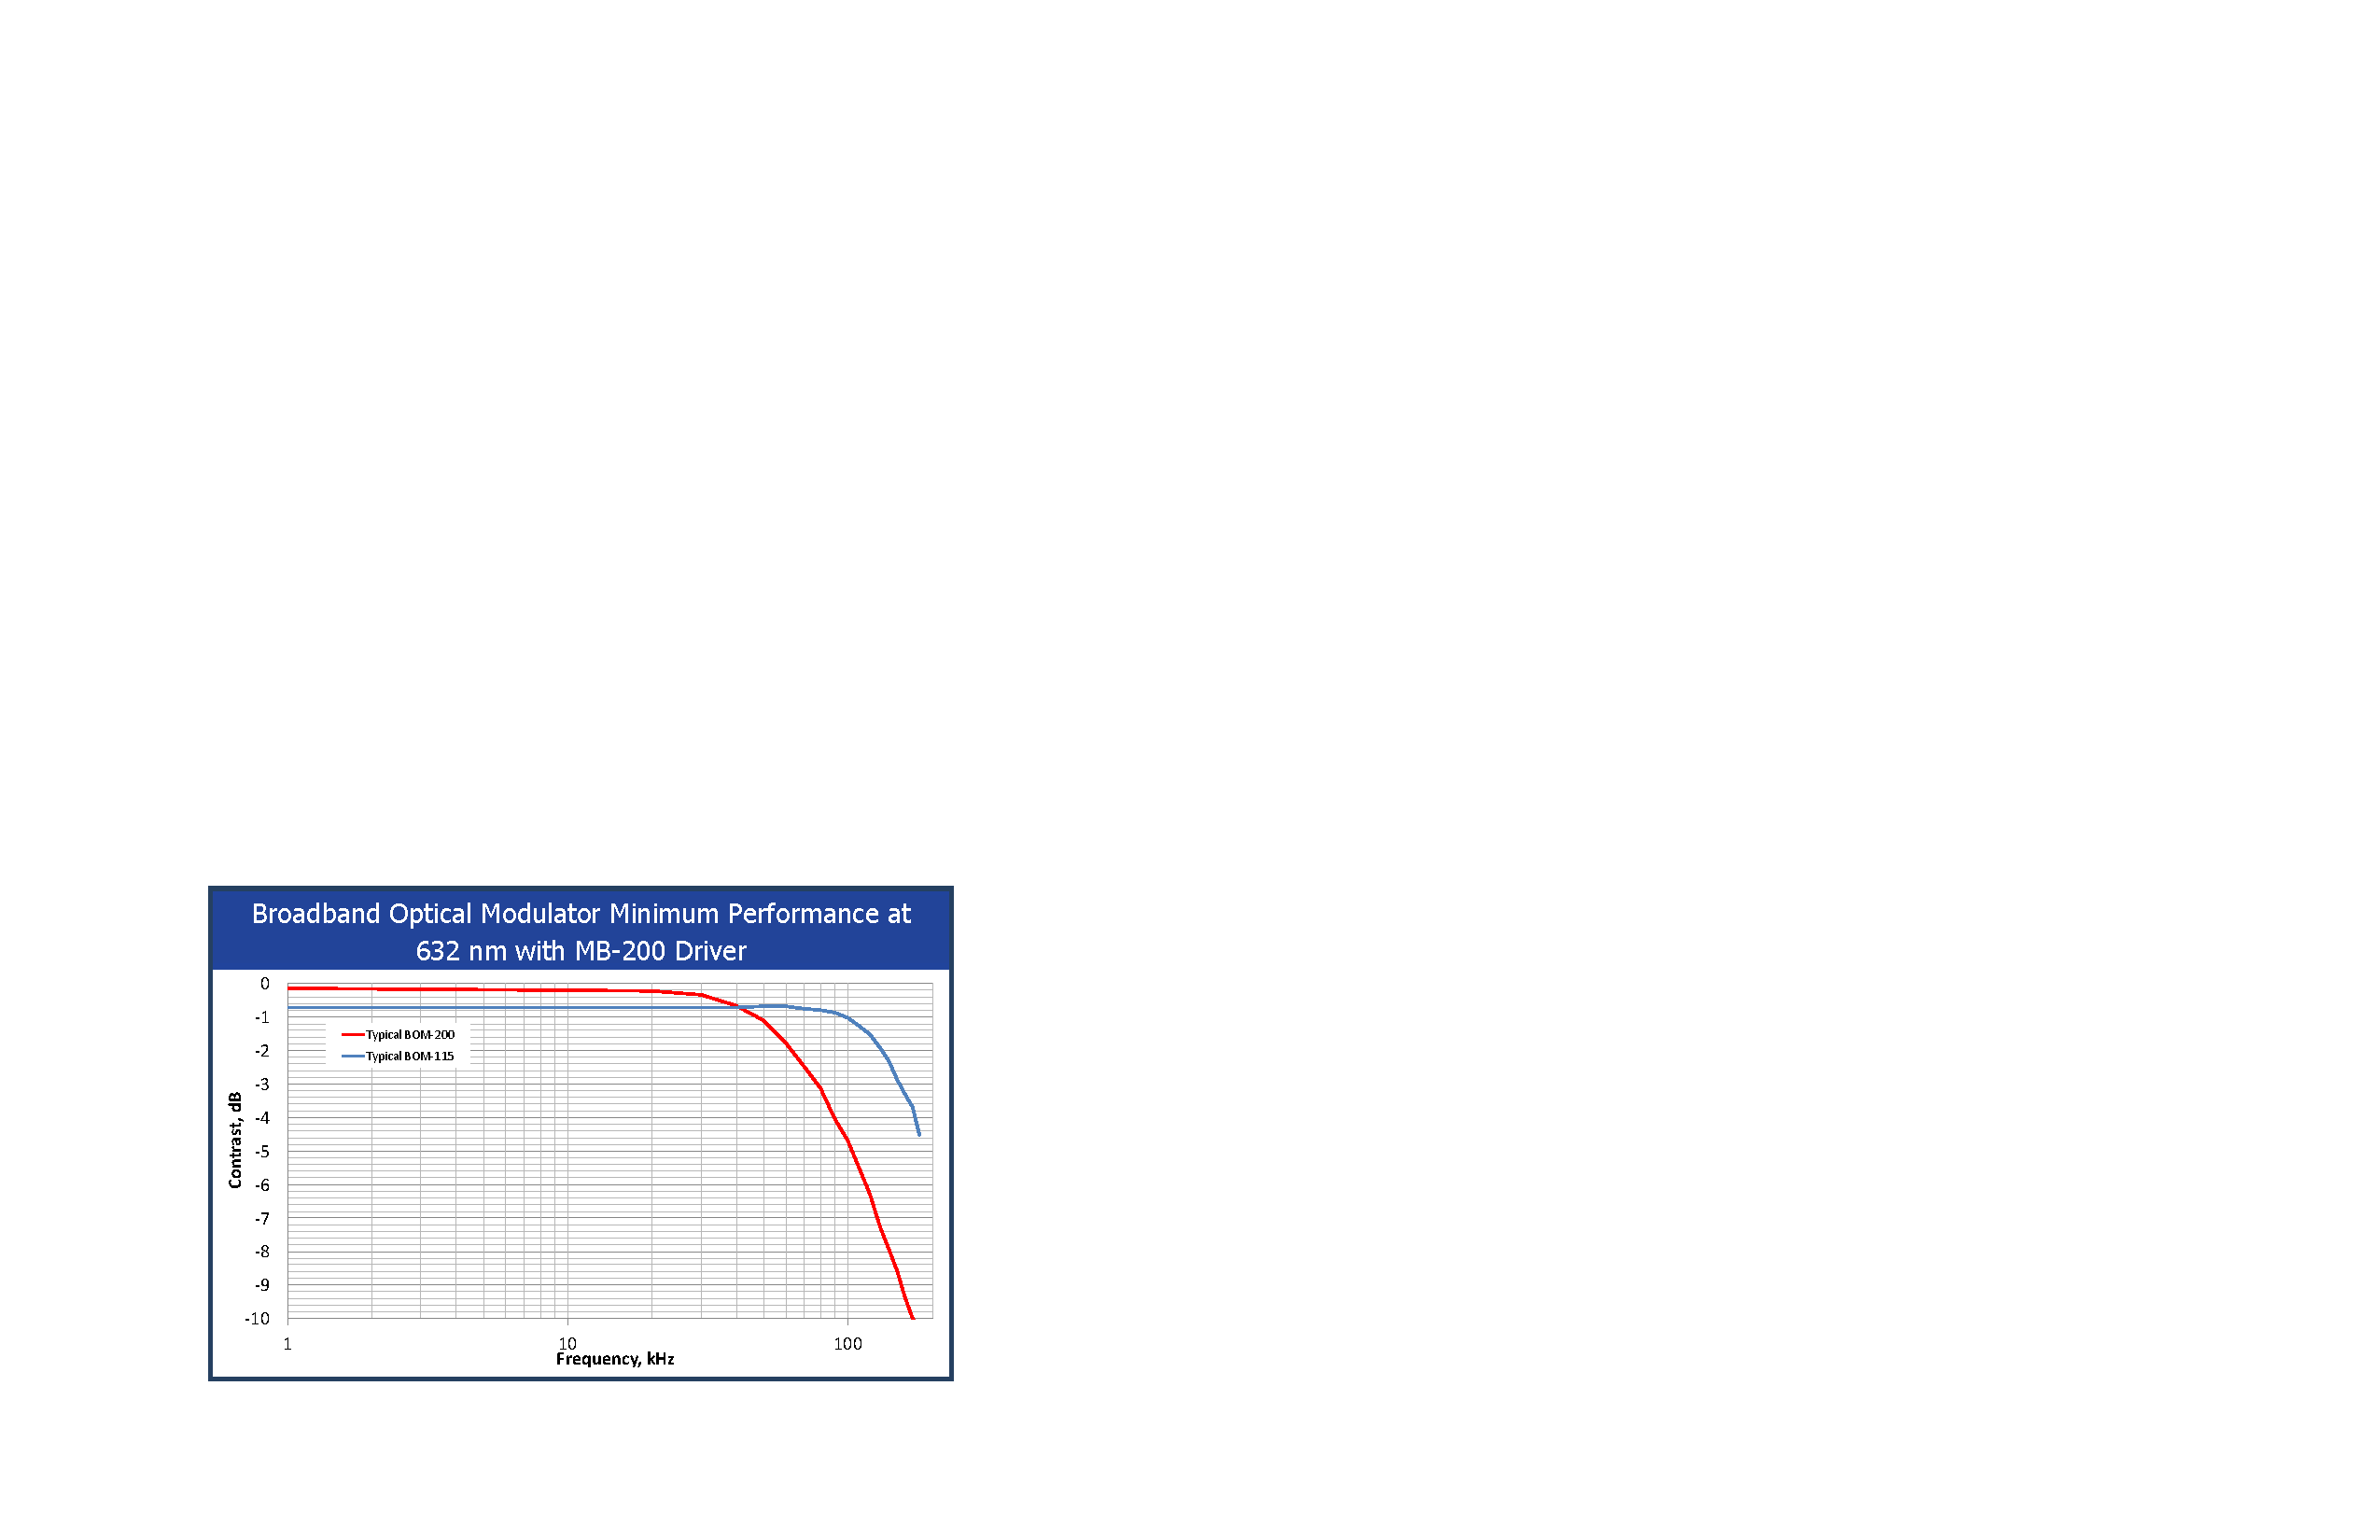
\includegraphics[width=\textwidth]{./Img/MB-200-frequency.pdf}
	\caption{}
	\label{fig:MB-200-frequency.pdf}
\end{subfigure}
	\bicaption{MEMS逆光调制器。(a) MEMS逆向调制器内部结构图,(b) MEMS逆向调制器外形图,(c)MEMS MRR驱动器,(d) MB-200的带宽}{MEMS MRR.(a) MEMS-MRR-INNER . (b) MEMS-MRR-OUTSIDE .(c)MEMS-MRR-driver.(d)Broadband Optical Modulator Minimum Performance at
		632 nm with MB-200 Driver.}
	\label{fig:MEMS-MRR-FIGURE}
\end{figure}

MRR系统已被证明能够使用二进制调制方案以高达200kbps的数据速率提供连续的非对称自由空间光通信。MRR可以与MB-200驱动器配对,支持使用标准5V的TTL电平进行测试光学测试,具体的驱动器参数如表~\ref{tab:MB-200}。

% Table generated by Excel2LaTeX from sheet 'Sheet1'
\begin{table}[htbp]
	\centering
	\caption{MB-200驱动器详细参数}
	\begin{tabular}{p{13.665em}p{11.335em}}
		\Xhline{1.2pt}
		\multicolumn{1}{l}{MB-200驱动器规格} & \multicolumn{1}{l}{参数} \\
		\Xhline{0.6pt}
		驱动器工作频率范围 & 0\textasciitilde300 kHz \\
		外壳尺寸  & $127\times101.6\times25.4 $mm \\
		电源供电电压 & 100\textasciitilde240V AC \\
		\Xhline{1.2pt}
	\end{tabular}%
	\label{tab:MB-200}%
\end{table}%



\subsection{MEMS MRR的机电特性}
MEMS逆向光调制器的电极最大横向距离为185$\mu$m,最大垂直位移为185$\mu$m。对比度的计算公式为
$$ \text{modulation contrast} = \dfrac{\text{PDVmax}–\text{PDVcurrent}}{\text{PDVmin}+\text{PDVmax}}  $$
式中PDV表示光电探测器的输出电压。

\begin{figure}[!htbp]
	\centering
	\begin{subfigure}[c]{0.5\textwidth}
		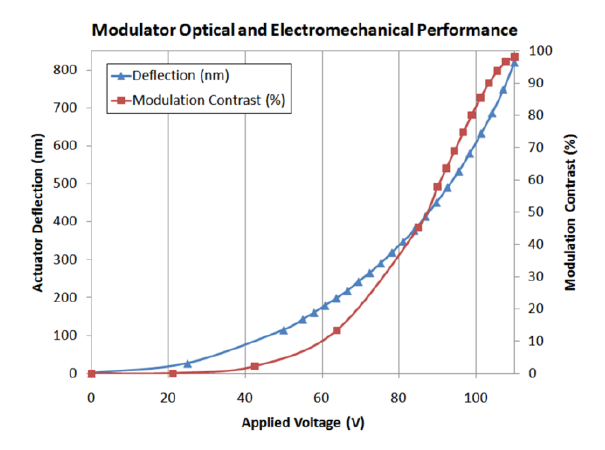
\includegraphics[width=\textwidth]{./Img/MEMS-MRR-VOLTAGE.png}
		\caption{}
		\label{fig:MEMS-MRR-VOLTAGE.png}
	\end{subfigure}%
	~%add desired spacing
	\begin{subfigure}[c]{0.6\textwidth}
		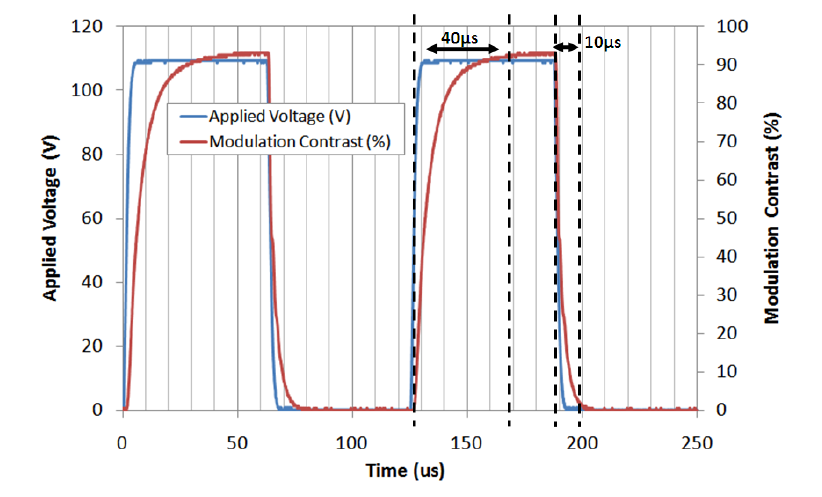
\includegraphics[width=\textwidth]{./Img/MEMS-MRR-RISETIME.png}
		\caption{}
		\label{fig:MEMS-MRR-RISETIME.png}
	\end{subfigure}
	\bicaption{MEMS逆光调制器。(a) 不同电压下的对比度和制动器位移,(b) 加载8kHz的方波,幅值为0\textasciitilde 110V的调制信号后,0级衍射条纹的动态响应。}{MEMS MRR.(a) Actuator deflection and modulation contrast behavior for a 200μm pitch modulator with an 185μm span.  (b) Dynamic response of the 185um span modulator to a 0 to 110V, 8kHz square wave, as seen by the photo detector	measuring the 0th diffraction order. }
	\label{fig:MEMS-MRR-table}
\end{figure}

从图~\ref{fig:MEMS-MRR-VOLTAGE.png}可以看出当施加电极两端电压为110V时,对比度已达到98\%,继续增大电压并不会使对比度再有大的提高。

从图~\ref{fig:MEMS-MRR-RISETIME.png}可以看出,当用8kHz,幅值为110V电压驱动MEMS MRR时,其阶跃响应为过阻尼。调制器对比度达到50\%时,需要的时间为7$\mu$s,达到98\%时,需要的时间为40$\mu$s,所以对应的最大工作频率为
$$f = \dfrac{1}{40\mu s}= 25 kHz$$


% Table generated by Excel2LaTeX from sheet 'Sheet1'
\begin{table}[htbp]
	\centering
	\caption{MEMS MRR详细参数}
	\begin{tabular}{p{13.665em}p{11.335em}}
		\Xhline{1.2pt}
		\multicolumn{1}{l}{MEMS MRR规格} & \multicolumn{1}{l}{参数} \\
		\Xhline{0.6pt}
		对比度 & >50\% Peak Contrast \\
		安装孔径  & 25.4 mm \\
		反射材料 & 金膜 \\
		光束偏转角 & <30 arcsec\\
		& $\left( 1~ \text{arcsec} = 1/3600 ^{\circ}  \right) $\\
		\Xhline{1.2pt}
	\end{tabular}%
	\label{tab:MRR}%
\end{table}%

\addimg{0.5}{MRR-ASSEMBLED.png}{MRR样机}
\addimg{1}{MRR-Incident-beam-angle-FOV.png}{MRR入射角和视场关系}

图~\ref{MRR-ASSEMBLED.png}展示了MRR样机模型;图~\ref{MRR-Incident-beam-angle-FOV.png}描述了MRR调制器的入射角和视场关系。
